\documentclass[10pt,a4paper, table]{article}
\usepackage[top=1.36in, bottom=1.36in, left=0.98in, right=0.98in]{geometry}
\usepackage[utf8]{inputenc}
\usepackage[czech]{babel}
\usepackage{tikz}
\usepackage{pgfplots}
\usepackage{xcolor,listings}
\usepackage{textcomp}
\usepackage{hyperref}
\usepackage{graphicx}
\usepackage{amsmath}
\usepackage{algorithm}
\usepackage{listings}
\usepackage{fontspec,minted}
\usepackage{subfig}
\usepackage{xevlna}

\title{Analýza obrazu II//Detekce parkovacích míst}
\author{Richard Zvonek}


\definecolor{backcolour}{rgb}{0.1686,0.1686,0.1686}

\newminted{c++}{
  style=monokai,,
  bgcolor=backcolour,
  fontsize=\small,
  frame=lines
}

\setmonofont{[JetBrainsMono-Regular.ttf]}[Contextuals=Alternate,Ligatures=TeX]


\begin{document}

\begin{center}
  {\Large Vysoká Škola Báňská – Technická Univerzita Ostrava\par
    Fakulta Elektrotechniky a Informatiky\par
    Katedra Informatiky\par}
  \vspace{26mm}
  {\Huge\bfseries Analýza obrazu II \par}
  \bigskip
  {\Huge\bfseries Detekce obsazenosti parkovacích míst \par}
\end{center}
\vfill
{\Large\number\year\hfill Richard Zvonek, ZVO0016}
\cleardoublepage

\newpage

\tableofcontents

\newpage

\section{Zadání}
Na zadaných testovacích datech detekovat obsazenost parkovacích míst, vyzkoušet metody s trénováním, bez trénování a srovnat výsledky. Pro srovnání výsledků vypsat počet nesprávně určených (false positive, false negative) výsledků a F1 score.\par
Testovací sada obsahuje 24 fotografií parkovacích míst, obsahující různě zaplněné parkoviště v různé denní doby.

\begin{figure}[ht]%
  \centering
  \subfloat[Testovací obraz]{{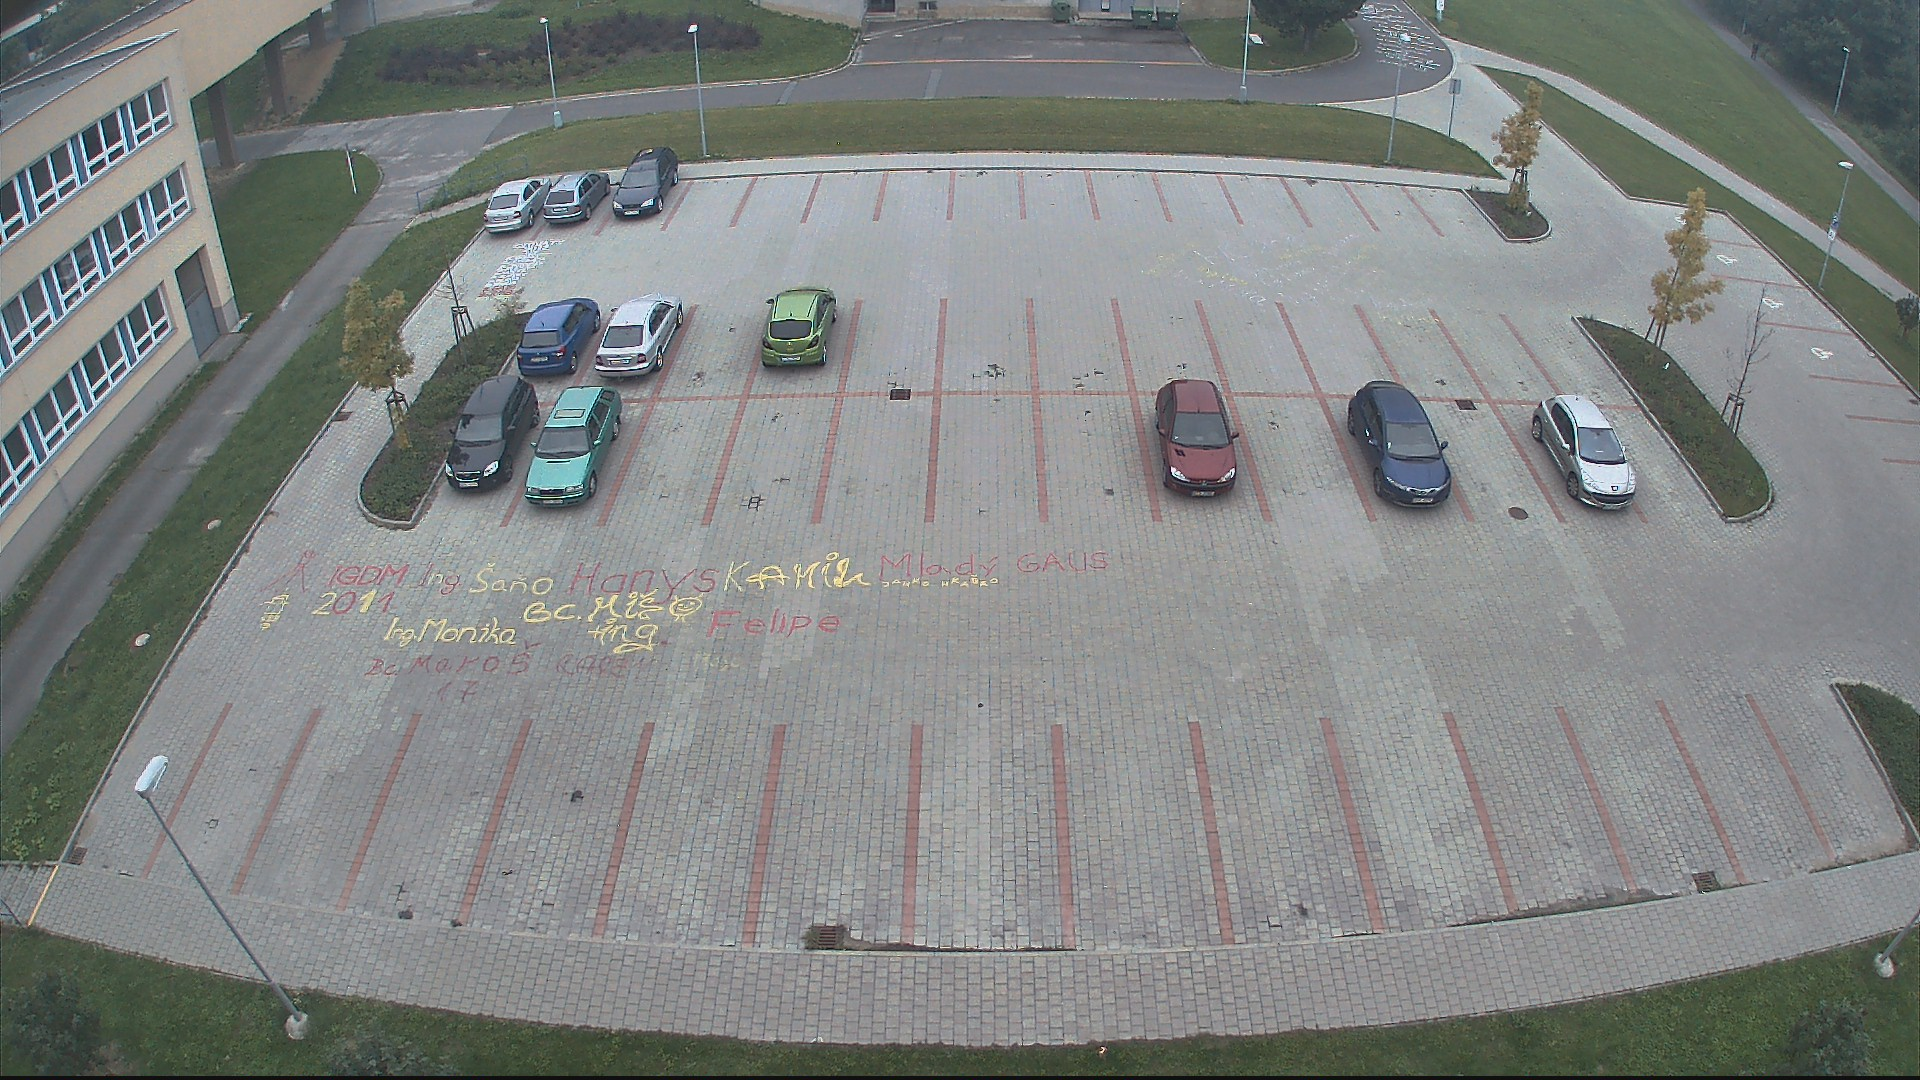
\includegraphics[width=10cm]{images/test10.jpg} }}%
  \qquad
  \subfloat[Noční testovací obraz]{{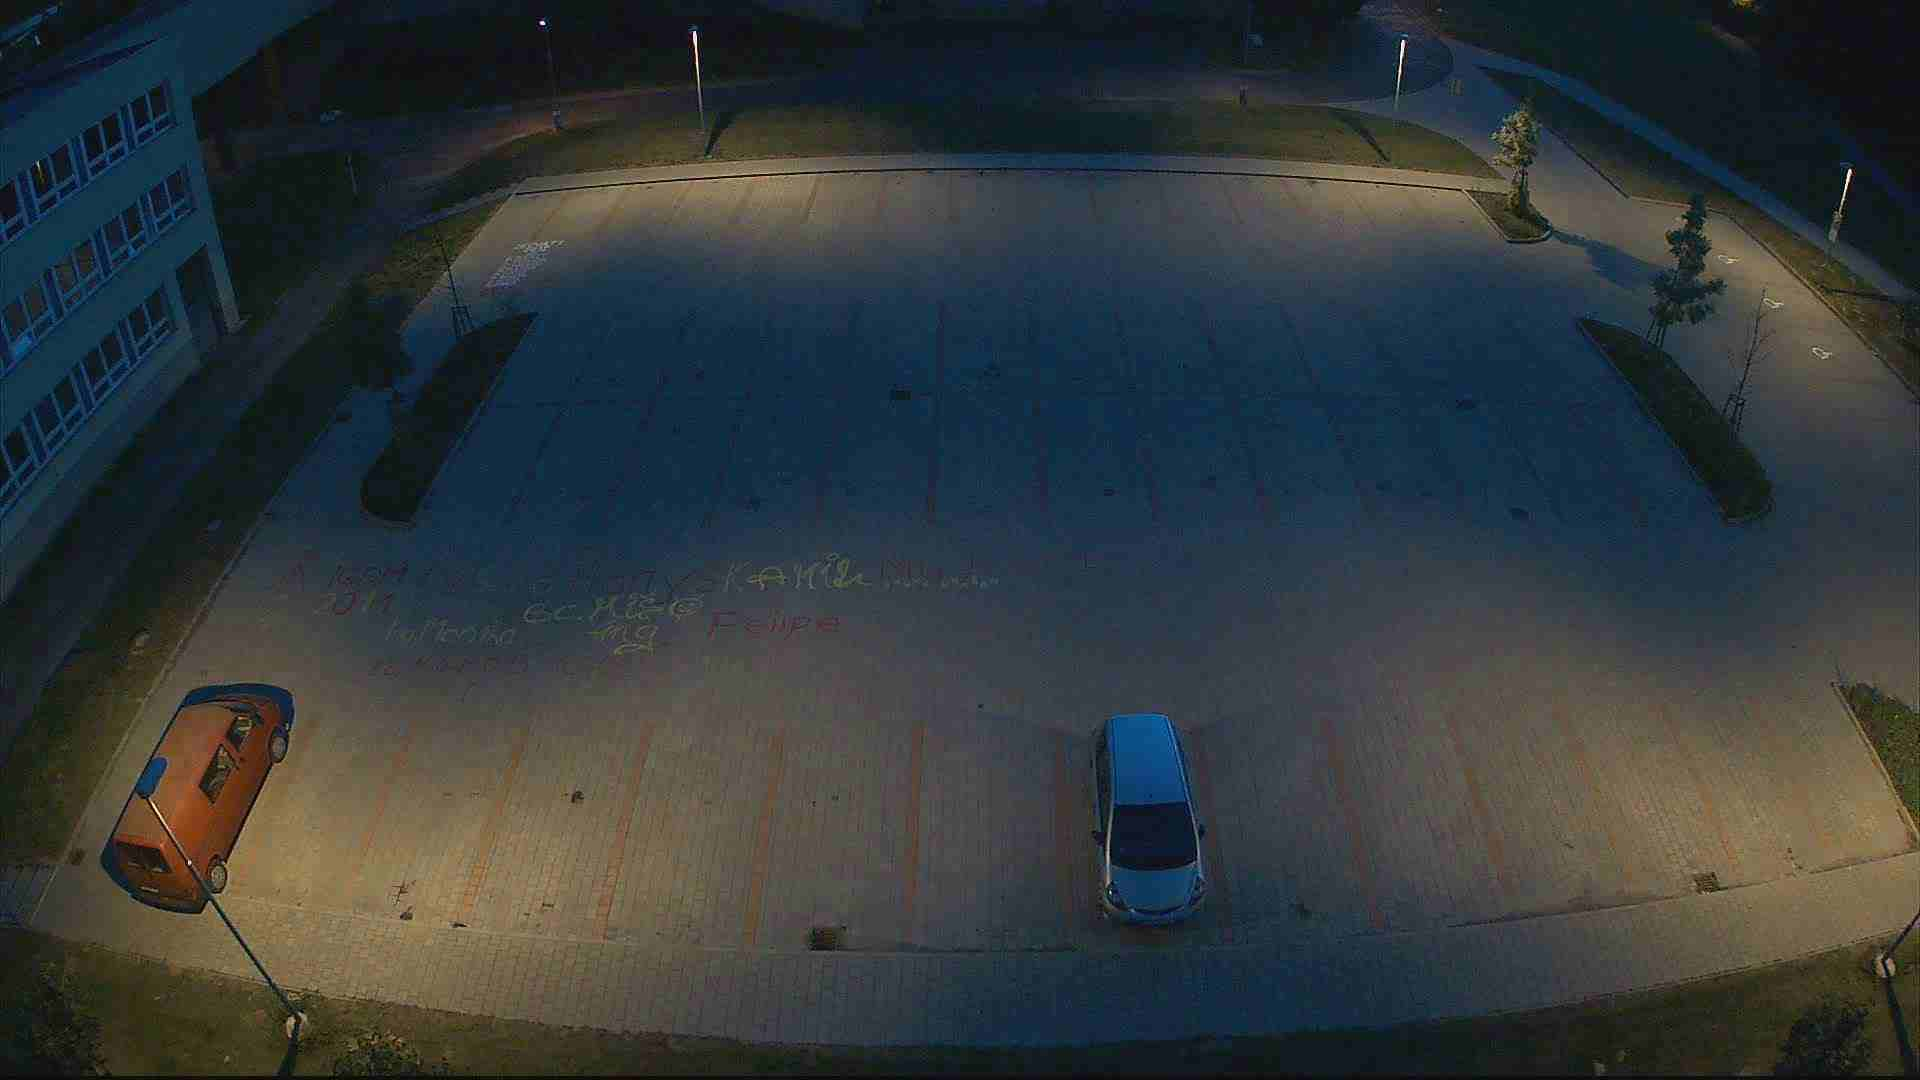
\includegraphics[width=10cm]{images/test15.jpg} }}%
  \qquad

  \caption{Ukázka testovacích obrazů}%
  \label{fig:testData}%
\end{figure}

\section{Detekce bez trénování}
Pro detekci bez trénování jsem vyzkoušel několik různých metod rozpoznávání. Kromě nejúspěšnější a nejjednodušší metody pomocí \hyperref[sec:canny]{Cannyho detektoru hran (viz \ref{sec:canny})} jsem vyzkoušel i variaci se stejným postupem s jinými detektory hran (Sobelův operátor, Laplace). Canny se osvědčil jako nejlépe fungující, proto jej dále rozvedu. Kromě těchto jednoduchých metod jsem rozpracoval i HAAR a HOG, ale HAAR jsem dále neimplementoval a HOG jsem nakonec nedokončil a zůstal v rozpracovaném stavu.

\subsection{Rozpoznávání pomocí detektoru hran} \label{sec:canny}
Nejjednodušší, nejméně náročnou a nejrychleji naimplementovanou metodou vůbec se stalo jednoduché rozpoznávání za pomocí detektorů hran. Po testování různých detektorů jsem nakonec použil Cannyho detektor, pro získání minimální a maximální hodnoty jsem nejprve volil empiricky zvolené metody, později jsem se uchýlil k automatickému výpočtu těchto hodnot pomocí OTSU prahování histogramem. Pro zvýšení úspěšnosti detektoru bylo potřeba vyladit předzpracování obrazu, nejvíce se mi osvědčila metoda rozmazání obrazu mediánem. Vyzkoušel jsem také úpravu jasu lineárně nebo pomocí histogramu, ale tyto metody nevedly ke zvýšení úspěšnosti detektoru.\par
Po získání obrazu z detektoru je potřeba použít nějakou metriku pro určení, zda je parkovací místo obsazeno nebo ne. V mém případě jsem vyzkoušel dva přístupy. V prvním přístupu jsem hledal horizontální a vertikální hrany pomocí Hough transformation \footnote{\url{https://www.learnopencv.com/hough-transform-with-opencv-c-python/}}, ve druhém přístupu jsem jednoduše spočítal počet bílých a černých pixelů, vypočítal jsem jejich podíl a podle něj jsem rozhodl, jestli je dané místo obsazeno nebo ne. Překvapivě se druhý způsob ukázal jako poměrně přesný, po částečně empirickém upravování hraničních hodnot\footnote{Vyexportoval jsem poměry a analyzoval jsem distribuci hodnot} jsem dosáhnul relativně kompetetivního score (viz \hyperref[tab:dnnResults]{tabulka \ref{tab:dnnResults}}). Nakonec jsem se rozhodl použít pouze tento jednoduchý způsob a detekci horizontálních a vertikálních hran jsem zahodil.

\section{Detekce s trénováním}
Při práci s detektory jsem narazil na potřebu mít modulární zdrojový kód, takže jsem vědoval několik hodin usilovnému refactoringu, až jsem došel k poměrně péknému objektovému, obecnému kódu. Definice nové neuronové sítě je tak práce na pár minut a jen pár řádků kódu. Pro samotné neuronové sítě jsem použil framework dlib, která potřebuje veškerou nutnou funkcionalitu. Při zprovoznění knihovny jsem nejprve neměl žádné problémy, ale celkové trénování a rozpoznávání bylo zoufale pomalé. Tato vlastnost byla způsobena nejen mým ne úplně high end vybavením, ale primárně  nepoužíváním CUDA. Po rekompilaci dlib s CUDA mi dlib přestal fungovat úplně z důvodu nesprávně nastavených ovladačů pro CUDA v arch linuxu. Následoval můj pokus o přeinstalaci ovladačů, který ovšem skončil nenaběhnutím systému. Pokračoval jsem tedy na čerstvě reinstalovaném linuxu, na kterém už bylo rozběhnutí dlib s CUDA otázkou chvilky. \par
Při pokusech s neuronovými sítěmi jsem narazil na některé nedostatky dodané tréninkové sady, které dále rozebírám v \hyperref[sec:augment]{kapitole \ref{sec:augment}}. Samotné použití neuronových sítí bylo nakonec celkem jednoduché, každou neuronovou síť jsem několikrát přetrénoval, každým tréninkem jsem dosáhl jiné úspěšnosti. Do celkových výsledků počítám nejlepší výsledek, každá nejlépe natrénovaná neuronová síť je pak uložena v přiloženém souboru.

\subsection{Trénovací data}\label{sec:augment}
Pro trénování neuronových sítí byly dodány trénovací obrazy prázdných a plných parkovacích míst. Nevýhodou dodaných trénovacích dat je absence nočních snímků. Na tento nedostatek neuronové sítě trpěly, proto jsem se rozhodl implementovat umělé rozšíření datové sady. Pro výpočet rozšíření datové sady jsem využil vysoce sofistikovaného postupu, viz \hyperref[lst:extendedImagesAlgo]{výpis \ref{lst:extendedImagesAlgo}}. Po rozšíření trénovací sady se celkový počet trénovacích dat zosminásobil, ukázka výsledku rozšíření je zobrazen na \hyperref[fig:testData]{obrázcích \ref{fig:testData}}. \par
Po aplikaci rozšíření se zvýší doba trénování neuronové sítě, zvýší se paměťová náročnost GPU při tréninku, ale celková přesnost se podstatně zvýší (v řádu jednotek procent).

\begin{listing}[ht]
\begin{c++code}
void TrainInputSet::getExtendedImages(const cv::Mat &inputImg,
std::vector<cv::Mat> &extendedImages) {
    cv::Mat flippedx;
    cv::Mat flippedy;
    cv::Mat flippedxy;

    cv::flip(inputImg, flippedx, 0);
    cv::flip(inputImg, flippedy, 1);
    cv::flip(inputImg, flippedxy, -1);

    extendedImages.emplace_back(flippedx);
    extendedImages.emplace_back(flippedy);
    extendedImages.emplace_back(flippedxy);

    // Simulate night
    extendedImages.emplace_back(inputImg / 2);
    extendedImages.emplace_back(flippedx / 3);
    extendedImages.emplace_back(flippedy / 4);
    extendedImages.emplace_back(flippedxy / 5);
  }
\end{c++code}
\caption{Výpočet rozšíření datové sady}
\label{lst:extendedImagesAlgo}
\end{listing}

\subsection{Použité neuronové sítě}
\subsubsection{LeNet}
LeNet síť jsem implementoval podle příkladu přímo od autorů knihovny dlib. Tato síť má v některých případech problémy s ostrými stíny, případně s nočním, silně zašumným obrazem. Dalším problémem je také nesprávné rozpoznání pouličního osvětlení jako zaplněného parkovacího místa, viz \hyperref[fig:dementniLampa]{obrázek \ref{fig:dementniLampa}}.\par
LeNet síť se dále vyznačovala rychlým tréninkem.

\begin{figure}[h]
  \centering
  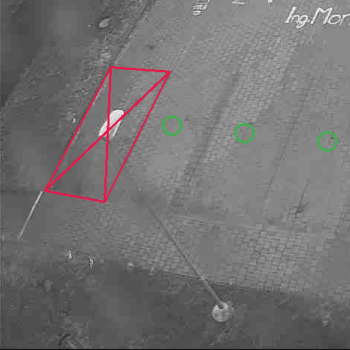
\includegraphics[width=5cm]{images/dementniLampa.png}
  \caption{Ukázka nesprávně rozpoznané lampy}%
  \label{fig:dementniLampa}%
\end{figure}

\subsubsection{AlexNet}
AlexNet síť jsem implementoval podle příkladu uvedeného na cvičení. Oproti klasické síti AlexNet jsem na vstup nedal obraz o velikosti 227x227, ale použil jsem nezměněný obraz 80x80. K této úpravě jsem se uchýlil po obtížích s tréninkem sítě, kty i při malých dávkách jsem měl problémy s nedostatečnou velikostí paměti a případně s velmi dlouhým tréninkem. Po znížení velikosti vstupního obrazu jsem už s natrénováním neměl problém, přestože se tato síť ze všech vyzkoušených řad k těm s řádově nejvyšší dobou tréninku. \par
Oproti síti LeNet nemá tato síť problémy s nočními snímky, ale sdílí problém s nesprávným rozpoznáváním lampy (viz viz \hyperref[fig:dementniLampa]{obrázek \ref{fig:dementniLampa}}), případně s parkovacími místy, které jsou opticky zakryta vozidly z vedlejšího parkovacího místa, viz \hyperref[fig:optickePrekryti]{obrázek \ref{fig:optickePrekryti}}.

\begin{figure}[h]
  \centering
  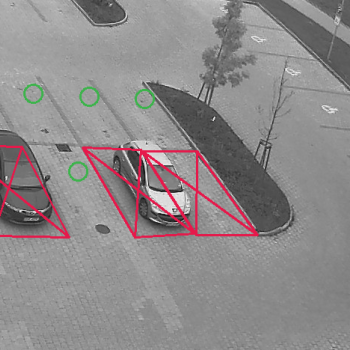
\includegraphics[width=5cm]{images/optickePrekryti.png}
  \caption{Ukázka opticky překrytého parkovacího místa }%
  \label{fig:optickePrekryti}%
\end{figure}
\subsubsection{VGG19}
Síť Vgg19 jsem implementoval podle příkladu uvedeného na cvičení. Oproti předchozím sítím se podstatně déle trénuje a nedosahuje lepších výsledků. Také je velmi hladová na systémové prostředky, i při rozlišení vstupu 32x32 jsem měl problémy s nedostatkem paměti. Předpokládám, že při hlubším zkoumání bych byl určitě schopen tuto síť odladit, ale vzhledem k dlouhým trénovacím časům jsem ji dále netestoval. Síť VGG19 v mnou natrénovaném stavu má podobné nedostatky, jako síť LeNet.

\subsubsection{ResNet}
Síť ResNet jsem implementoval podle příkladu na stránkách dlib. Při prvním spuštění jsem byl přkvapen, protože při trénovacím čase srovnatelným s LeNet dosahovala tato síť drasticky lepších výkonů. Tato síť je schopna spolehlivě rozpoznávat i na částečně překrytých místech a eliminuje i některé detekce lamp. Ne však všechny.

\subsubsection{GoogLeNet}
Síť GoogLeNet oproti ResNet překvapuje ještě lepším časem tréninku se srovnatelným výkonem při rozpoznávání. Problémem je opět lampa a v některých případech i částečné překrytí parkovacího místa.

\section{Kombinované rozpoznávání}
Pro zvýšení přesnosti jsem implementoval kombinace jednotlivých rozpoznávacích metod. Až na kombinaci všech metod ale nebyly kombinace o tolik lepší, než samotné nejlepší neuronové sítě, proto se o nich zmíním jen krátce.

\subsection{Kombinace AlexNet, ResNet a GoogLeNet}
Vzhledem k tomu, že v některých případech měly kombinované sítě nedostatky v různých oblastech, očekával jsem, že se tyto nedostatky vyeliminují. To se ovšem úplně nestalo, kombinace těchto tří sítí není lepší, než nejlepší z nich.

\subsection{Kombinace všech rozpoznávacích metod}
Jednou z nejlepších kombinací je kombinace všech metod rozpoznávání. Rozpoznání se přijme, pokud se na výsledku shodne 4 z 5 sítí. Tato kombinace dosahuje úplně nejlepších výsledků, ale také je časově nejnáročnější.

\clearpage
\section{Závěr}
Naimplementoval jsem různé metody pro rozpoznávání obsazenosti parkoviště, výsledné srovnání je přiloženo v \hyperref[tab:dnnSetting]{tabulce \ref{tab:dnnSetting}} a \hyperref[tab:dnnResults]{\ref{tab:dnnResults}}. Zdrojové kódy jsou k dispozici na \url{https://github.com/SacrificeGhuleh/ANOII2020/tree/ANOII2020} (je třeba rekurzivní git clone z důvodu použití submodulu), pro build je potřeba cmake. Využívám některé funkce z C++17, je tedy potřeba mít kompatibilní kompilátor. Testoval jsem funkčnost na gcc v10.2.0. Na \url{https://github.com/SacrificeGhuleh/ANOII2020/releases/tag/ANOII2020} je také možné stáhnout výsledky jednotlivých metod rozpoznávání v obrazové formě a binární soubory natrénovaných sítí (soubor ANOII.zip).\par
Co se týče samotných výsledků, nejlepší výsledek dává rozpznávání pomocí kombinace všech metod. Tato úspěšnost je však vykoupena mnohem vyšším časem, který je potřeba pro rozpoznání. Mými osobními favority se tak stávají sítě ResNet a GoogLeNet, které dosahují skvělých výsledků s nízkými časy trénování i rozpoznávání.

\clearpage
\section*{Přílohy}


\subsection*{Srovnání neuronových sítí}

\rowcolors{2}{gray!25}{white}

\begin{table}[h]
  \centering
  \begin{tabular}{r|lllllll}
    DNN                        &
    \begin{tabular}[c]{@{}l@{}}Velikost \\ obrazu\end{tabular}  &
    \begin{tabular}[c]{@{}l@{}}Learning \\ Rate\end{tabular}  &
    \begin{tabular}[c]{@{}l@{}}Min \\ Learning \\ Rate\end{tabular}  &
    \begin{tabular}[c]{@{}l@{}}Batch \\ size\end{tabular}  &
    \begin{tabular}[c]{@{}l@{}}Max steps \\ without progress\end{tabular}  &
    \begin{tabular}[c]{@{}l@{}}Max \\ epochs\end{tabular} &
    \begin{tabular}[c]{@{}l@{}}Doba \\ tréninku\footnotemark\end{tabular}   \\
    \hline
    LeNet                      &
    $28 \times 28$             &
    $0.01$                     &
    $10^{-6}$                  &
    $128$                      &
    $1000$                     &
    $300$                      &
    $\approx 45s$                \\

    AlexNet                    &
    $80 \times 80$             &
    $0.01$                     &
    $0.001$                    &
    $256$                      &
    $1000$                     &
    $300$                      &
    $800s \sim 1000s$            \\

    Vgg19                      &
    $32 \times 32$             &
    $0.01$                     &
    $10^{-7}$                  &
    $64$                       &
    $500$                      &
    $300$                      &
    $\approx 3000s$              \\

    ResNet                     &
    $32 \times 32$             &
    $0.01$                     &
    $10^{-7}$                  &
    $64$                       &
    $128$                      &
    $300$                      &
    $\approx 40s$                \\

    GoogLeNet                  &
    $32 \times 32$             &
    $0.01$                     &
    $10^{-7}$                  &
    $64$                       &
    $128$                      &
    $300$                      &
    $\approx 35s$                \\\hline
  \end{tabular}
  \caption{Nastavení neuronových sítí}
  \label{tab:dnnSetting}
  \centering
\end{table}


\footnotetext{Trénování a rozpoznávání bylo testováno na Manjaro Linux x86\_64 5.8.18, Intel i5-5200U@2.7GHz, NVIDIA GeForce GTX 850M, 4GB VRAM}
\begin{table}[h]
  \centering
  \begin{tabular}{r|lllllll}
    Metoda                     &
    \begin{tabular}[c]{@{}l@{}}False \\ positives\end{tabular} &
    \begin{tabular}[c]{@{}l@{}}False \\ negatives\end{tabular} &
    \begin{tabular}[c]{@{}l@{}}Přesnost \\ rozpoznání\end{tabular} &
    \begin{tabular}[c]{@{}l@{}}F1 \\ score\end{tabular}   \\
    \hline
    Canny                      &
    $91$                       &
    $0$                        &
    $0.932$                    &
    $0.965$                      \\

    LeNet                      &
    $25$                       &
    $0$                        &
    $0.981$                    &
    $0.990$                      \\

    AlexNet                    &
    $12$                       &
    $0$                        &
    $0.991$                    &
    $0.996$                      \\

    Vgg19                      &
    $26$                       &
    $0$                        &
    $0.981$                    &
    $0.990$                      \\

    ResNet                     &
    $11$                       &
    $0$                        &
    $0.992$                    &
    $0.996$                      \\

    GoogLeNet                  &
    $10$                       &
    $1$                        &
    $0.992$                    &
    $0.994$                      \\

    \begin{tabular}[r]{@{}r@{}}Kombinace: \\ AlexNet\\  ResNet \\ GoogLeNet\end{tabular} &
    $10$                       &
    $1$                        &
    $0.993$                    &
    $0.996$                      \\

    \begin{tabular}[r]{@{}r@{}}Kombinace: \\ všechny metody\\min$\frac{4}{5}$\end{tabular} &
    $5$                        &
    $0$                        &
    $0.996$                    &
    $0.998$                      \\



    \hline
  \end{tabular}
  \caption{Výsledky různých typů rozpoznávání}
  \label{tab:dnnResults}
  \centering
\end{table}


\clearpage
\subsection*{Rozšířená trénovací sada}
\newcommand\testImgWitdth{4cm}

\begin{figure}[ht]%
  \centering
  \subfloat[Originál]{{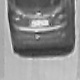
\includegraphics[width=\testImgWitdth]{images/1000_orig.jpg} }}%
  \qquad
  \subfloat[Překlopený obraz podle x]{{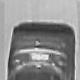
\includegraphics[width=\testImgWitdth]{images/1000flipx.jpg} }}%
  \qquad
  \subfloat[Překlopený obraz podle y]{{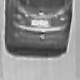
\includegraphics[width=\testImgWitdth]{images/1000flipy.jpg} }}%
  \qquad
  \subfloat[Překlopený obraz podle xy]{{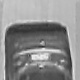
\includegraphics[width=\testImgWitdth]{images/1000flipxy.jpg} }}%
  \qquad
  \subfloat[Noční obraz s jasem $\frac{1}{2}$]{{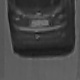
\includegraphics[width=\testImgWitdth]{images/1000_orig_night.jpg} }}%
  \qquad
  \subfloat[Noční obraz s jasem $\frac{1}{3}$]{{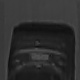
\includegraphics[width=\testImgWitdth]{images/1000flipx_night.jpg} }}%
  \qquad
  \subfloat[Noční obraz s jasem $\frac{1}{4}$]{{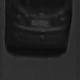
\includegraphics[width=\testImgWitdth]{images/1000flipy_night.jpg} }}%
  \qquad
  \subfloat[Noční obraz s jasem $\frac{1}{5}$]{{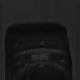
\includegraphics[width=\testImgWitdth]{images/1000flipxy_night.jpg} }}%
  \qquad

  \caption{Ukázka rozšířené trénovací sady}%
  \label{fig:testData}%
\end{figure}

\end{document}
